\documentclass[tikz,border=3pt]{standalone}
\usepackage[T1]{fontenc}
\usepackage{newtxtext,newtxmath}
\usetikzlibrary{arrows.meta,positioning,fit}
\begin{document}
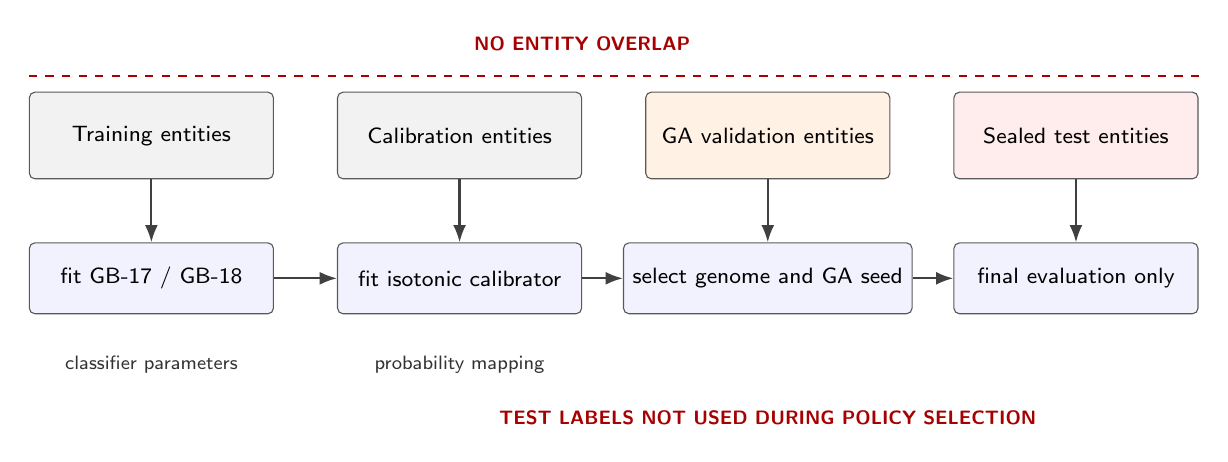
\begin{tikzpicture}[
  font=\sffamily\footnotesize,
  role/.style={draw=black!65, rounded corners=2pt, minimum width=31mm, minimum height=11mm, align=center},
  process/.style={draw=black!65, rounded corners=2pt, fill=blue!5, minimum width=31mm, minimum height=9mm, align=center},
  arrow/.style={-{Latex[length=2.2mm]}, thick, draw=black!75},
  guard/.style={font=\sffamily\scriptsize\bfseries, text=red!65!black, align=center},
  note/.style={font=\sffamily\scriptsize, align=center, text=black!80}
]
\node[role,fill=gray!10] (train) {Training entities};
\node[role,fill=gray!10,right=8mm of train] (cal) {Calibration entities};
\node[role,fill=orange!10,right=8mm of cal] (ga) {GA validation entities};
\node[role,fill=red!7,right=8mm of ga] (test) {Sealed test entities};
\node[process,below=8mm of train] (fit) {fit GB-17 / GB-18};
\node[process,below=8mm of cal] (isotonic) {fit isotonic calibrator};
\node[process,below=8mm of ga] (select) {select genome and GA seed};
\node[process,below=8mm of test] (evaluate) {final evaluation only};
\draw[arrow] (train)--(fit);
\draw[arrow] (cal)--(isotonic);
\draw[arrow] (ga)--(select);
\draw[arrow] (test)--(evaluate);
\draw[arrow] (fit)--(isotonic);
\draw[arrow] (isotonic)--(select);
\draw[arrow] (select)--(evaluate);
\node[guard,above=4mm of cal.north east, anchor=south] {NO ENTITY OVERLAP};
\draw[red!65!black,thick,dashed] ([yshift=2mm]train.north west) -- ([yshift=2mm]test.north east);
\node[guard,below=11mm of select.south] (testguard) {TEST LABELS NOT USED DURING POLICY SELECTION};
\node[note,below=4mm of fit] {classifier parameters};
\node[note,below=4mm of isotonic] {probability mapping};
\end{tikzpicture}
\end{document}
